\documentclass[border=15pt]{standalone}
\usepackage[utf8]{inputenc}
\usepackage[T1]{fontenc}
\usepackage{lmodern}
\usepackage{tikz}
\usetikzlibrary{shapes.geometric, arrows.meta, calc, backgrounds}

\definecolor{ambercolor}{RGB}{245, 197, 24}
\definecolor{skyblue}{RGB}{59, 155, 219}
\definecolor{navydark}{RGB}{13, 43, 85}
\definecolor{medblue}{RGB}{26, 94, 184}
\definecolor{indigoblue}{RGB}{58, 77, 184}
\definecolor{purplelight}{RGB}{230, 210, 250}
\definecolor{purpledark}{RGB}{100, 20, 160}
\definecolor{sysbg}{RGB}{235, 235, 235}
\definecolor{noteyellow}{RGB}{255, 253, 200}

\begin{document}
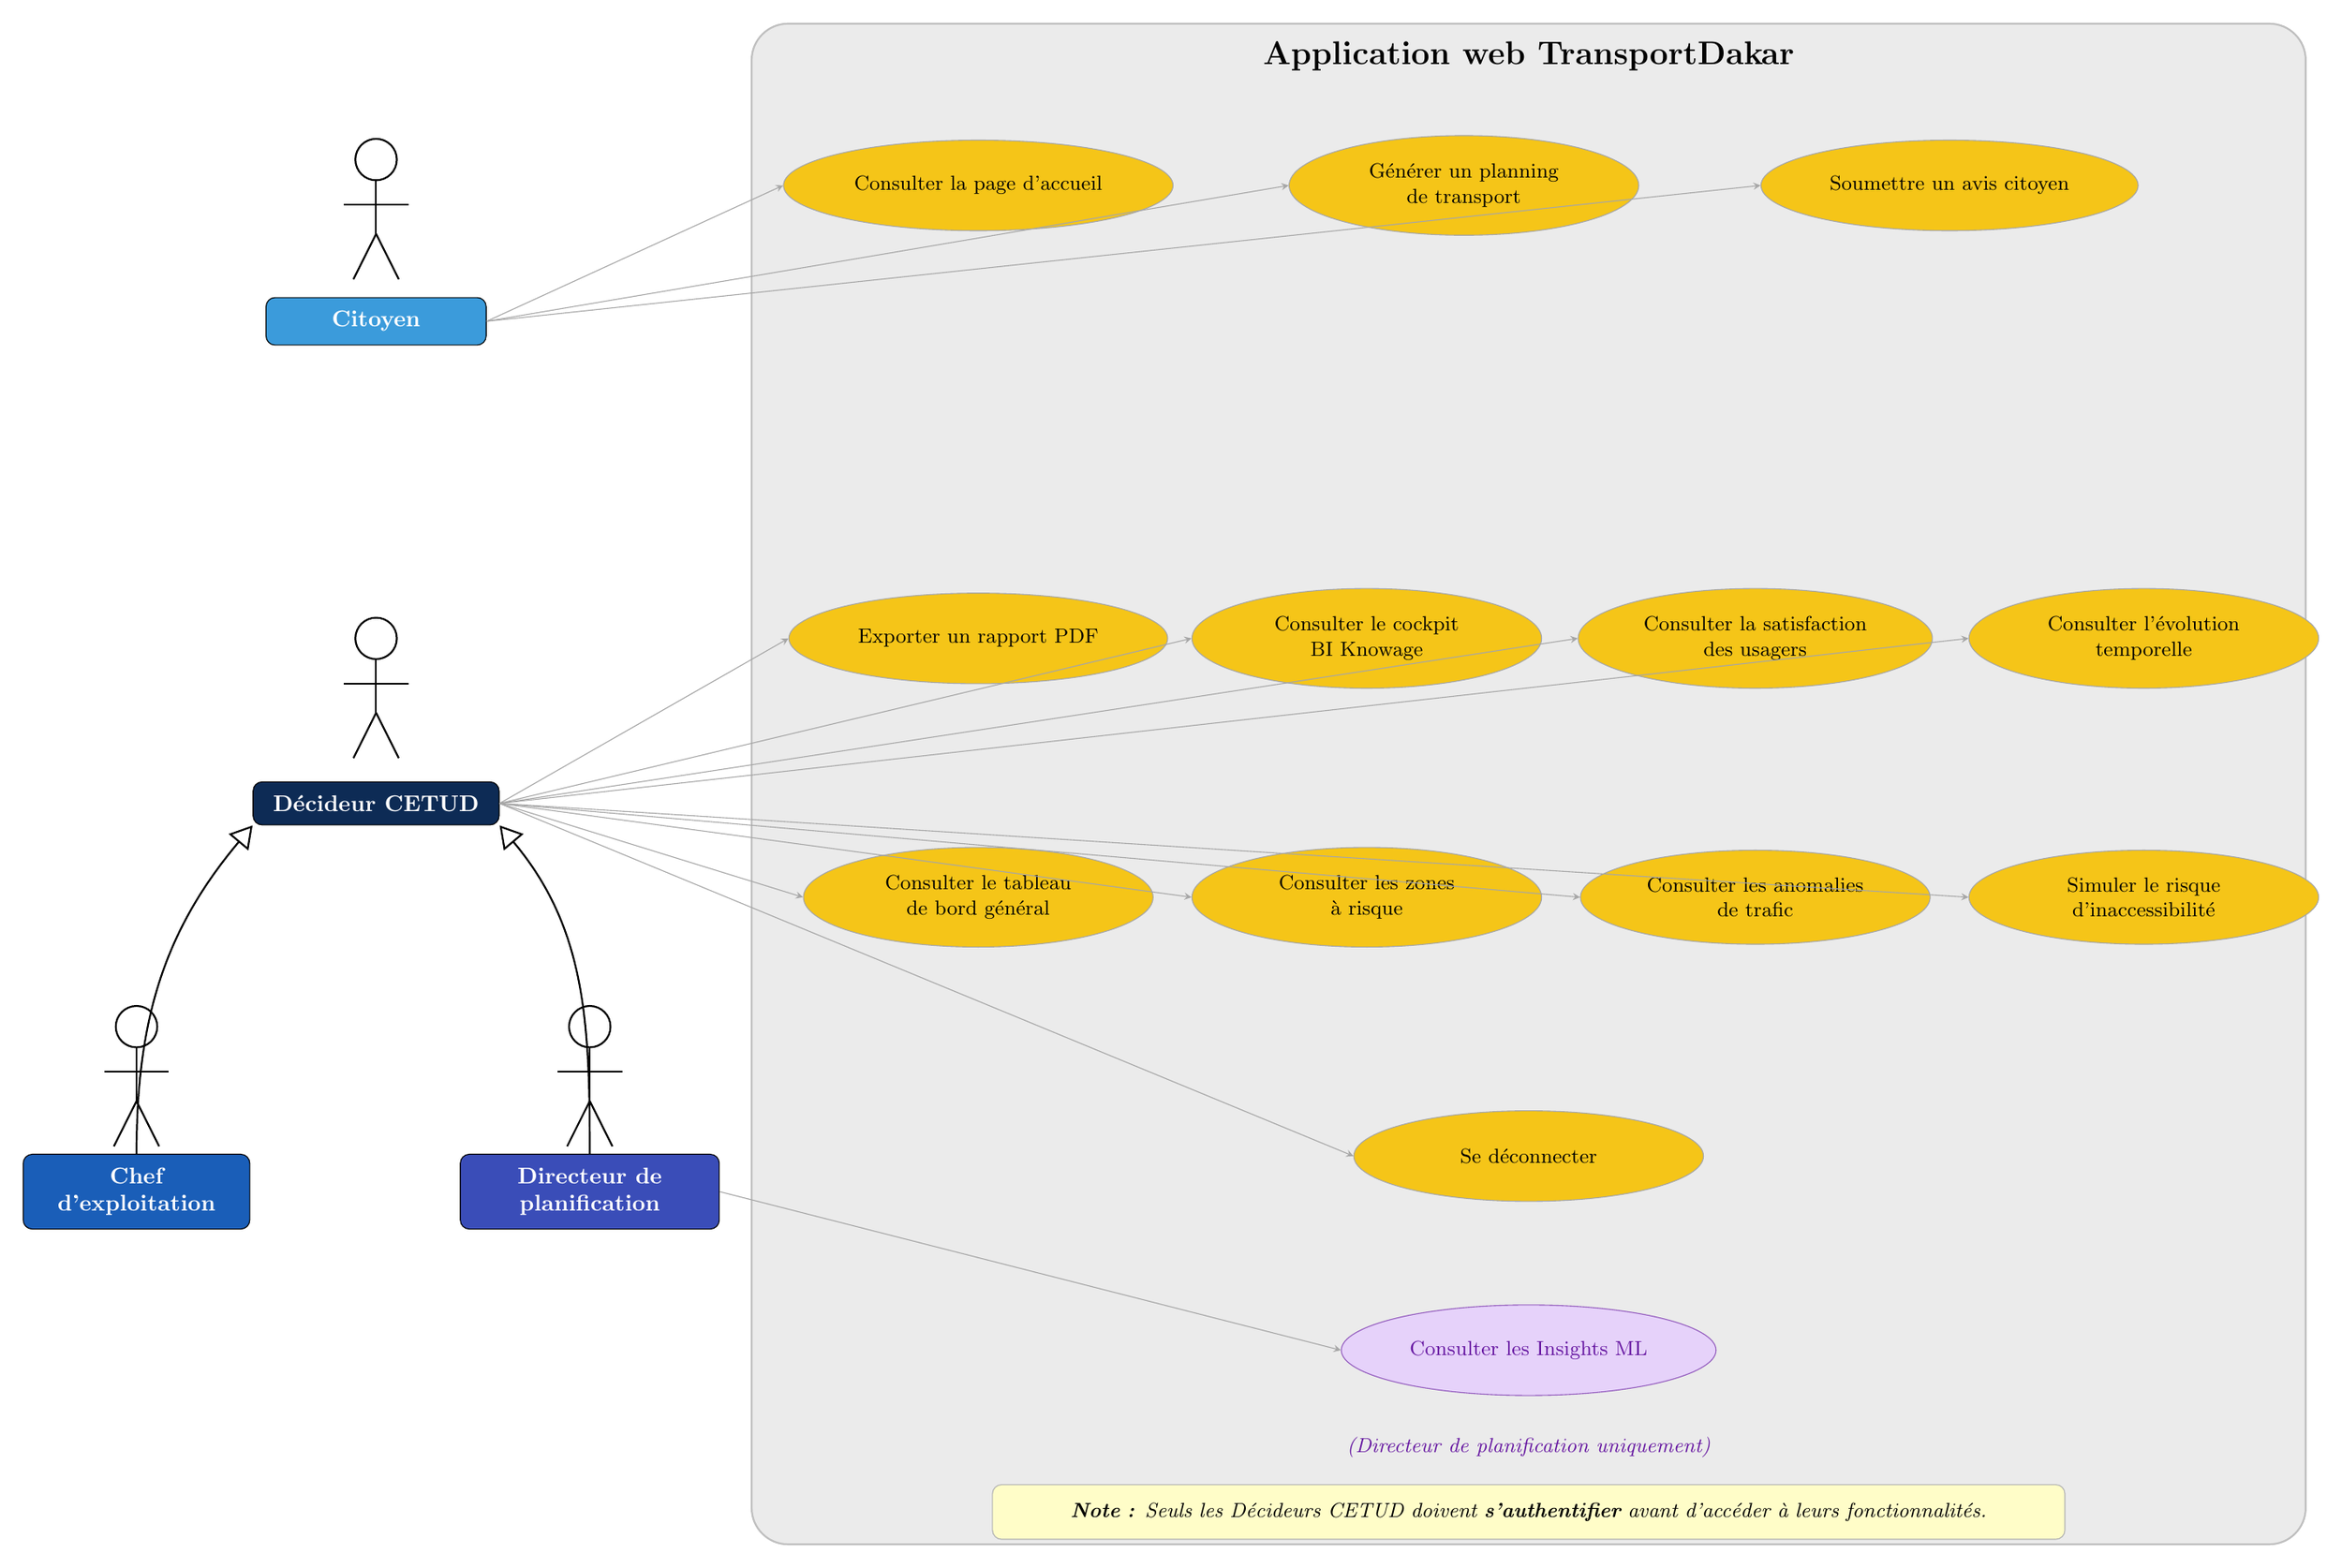
\begin{tikzpicture}[
  >=stealth, font=\normalfont,
  albl/.style={
    draw, rounded corners=4pt, text=white,
    font=\bfseries\normalsize,
    inner sep=6pt, align=center, minimum width=3.4cm
  },
  % Ellipses : taille controlée par minimum width/height, texte avec \\ explicites
  uc/.style={
    ellipse, draw=gray!70, fill=ambercolor,
    align=center, font=\small, inner sep=6pt,
    minimum width=5.4cm, minimum height=1.4cm
  },
  ucdir/.style={
    ellipse, draw=purpledark!70, fill=purplelight,
    text=purpledark, align=center, font=\small, inner sep=6pt,
    minimum width=5.4cm, minimum height=1.4cm
  },
  assoc/.style={->, thin, gray!70},
  gen/.style={-{Triangle[open, scale=2.0]}, thick, black}
]

% ══════════════════════════════════════════════════
% CADRE SYSTÈME  (commence à x=8.0)
% ══════════════════════════════════════════════════
\begin{scope}[on background layer]
  \draw[rounded corners=16pt, fill=sysbg, draw=gray!50, thick]
    (8.0, 1.5) rectangle (32.0, -22.0);
\end{scope}
\node[font=\Large\bfseries] at (20.0, 1.0)
  {Application web TransportDakar};

% ══════════════════════════════════════════════════
% ACTEURS — tous à x < 8, hors du cadre
% ══════════════════════════════════════════════════

%% Citoyen
\draw[thick] (2.2,-0.6) circle (0.32);
\draw[thick] (2.2,-0.92) -- (2.2,-1.75);
\draw[thick] (1.70,-1.30) -- (2.70,-1.30);
\draw[thick] (2.2,-1.75) -- (1.85,-2.45);
\draw[thick] (2.2,-1.75) -- (2.55,-2.45);
\node[albl, fill=skyblue] (Cit) at (2.2,-3.10) {Citoyen};

%% Décideur CETUD
\draw[thick] (2.2,-8.00) circle (0.32);
\draw[thick] (2.2,-8.32) -- (2.2,-9.15);
\draw[thick] (1.70,-8.70) -- (2.70,-8.70);
\draw[thick] (2.2,-9.15) -- (1.85,-9.85);
\draw[thick] (2.2,-9.15) -- (2.55,-9.85);
\node[albl, fill=navydark, minimum width=3.8cm] (Dec) at (2.2,-10.55)
  {D\'ecideur CETUD};

%% Chef d'exploitation  (x = -1.5, bien séparé à gauche)
\draw[thick] (-1.5,-14.00) circle (0.32);
\draw[thick] (-1.5,-14.32) -- (-1.5,-15.15);
\draw[thick] (-2.00,-14.70) -- (-1.00,-14.70);
\draw[thick] (-1.5,-15.15) -- (-1.85,-15.85);
\draw[thick] (-1.5,-15.15) -- (-1.15,-15.85);
\node[albl, fill=medblue, minimum width=3.5cm] (Chef) at (-1.5,-16.55)
  {Chef\\d'exploitation};

%% Directeur de planification  (x = 5.5, séparé à droite)
\draw[thick] (5.5,-14.00) circle (0.32);
\draw[thick] (5.5,-14.32) -- (5.5,-15.15);
\draw[thick] (5.00,-14.70) -- (6.00,-14.70);
\draw[thick] (5.5,-15.15) -- (5.15,-15.85);
\draw[thick] (5.5,-15.15) -- (5.85,-15.85);
\node[albl, fill=indigoblue, minimum width=4.0cm] (Dir) at (5.5,-16.55)
  {Directeur de\\planification};

%% Généralisations
\draw[gen] (Chef.north) to[out=90,in=230] (Dec.south west);
\draw[gen] (Dir.north)  to[out=90,in=310] (Dec.south east);

% ══════════════════════════════════════════════════
% CAS D'UTILISATION — Citoyen
% (3 UCs, espacés sur x = 11.5, 18.5, 25.5)
% ══════════════════════════════════════════════════
\node[uc] (UC1) at (11.5,-1.0) {Consulter la page d'accueil};
\node[uc] (UC2) at (19.0,-1.0) {G\'en\'erer un planning\\de transport};
\node[uc] (UC3) at (26.5,-1.0) {Soumettre un avis citoyen};

% ══════════════════════════════════════════════════
% CAS D'UTILISATION — Décideur CETUD (9 communs)
% 4 par ligne, x = 11.5, 17.5, 23.5, 29.5
% ══════════════════════════════════════════════════

%% Ligne 1
\node[uc] (UC4) at (11.5,-8.0) {Exporter un rapport PDF};
\node[uc] (UC5) at (17.5,-8.0) {Consulter le cockpit\\BI Knowage};
\node[uc] (UC6) at (23.5,-8.0) {Consulter la satisfaction\\des usagers};
\node[uc] (UC7) at (29.5,-8.0) {Consulter l'\'evolution\\temporelle};

%% Ligne 2
\node[uc] (UC8)  at (11.5,-12.0) {Consulter le tableau\\de bord g\'en\'eral};
\node[uc] (UC9)  at (17.5,-12.0) {Consulter les zones\\à risque};
\node[uc] (UC10) at (23.5,-12.0) {Consulter les anomalies\\de trafic};
\node[uc] (UC11) at (29.5,-12.0) {Simuler le risque\\d'inaccessibilit\'e};

%% Ligne 3 — Se déconnecter
\node[uc] (UC12) at (20.0,-16.0) {Se d\'econnecter};

% ══════════════════════════════════════════════════
% CAS D'UTILISATION — Directeur uniquement
% ══════════════════════════════════════════════════
\node[ucdir] (UC13) at (20.0,-19.0) {Consulter les Insights ML};
\node[font=\small\itshape, text=purpledark] at (20.0,-20.5)
  {(Directeur de planification uniquement)};

% ══════════════════════════════════════════════════
% NOTE — bas du cadre
% ══════════════════════════════════════════════════
\node[draw=gray!60, fill=noteyellow, rounded corners=4pt,
      inner sep=8pt, align=center, font=\small\itshape, text width=16cm]
  at (20.0,-21.5)
{
  \textbf{Note :} Seuls les D\'ecideurs CETUD doivent
  \textbf{s'authentifier} avant d'acc\'eder \`a leurs fonctionnalit\'es.
};

% ══════════════════════════════════════════════════
% FLÈCHES
% ══════════════════════════════════════════════════

%% Citoyen
\draw[assoc] (Cit.east) -- (UC1.west);
\draw[assoc] (Cit.east) -- (UC2.west);
\draw[assoc] (Cit.east) -- (UC3.west);

%% Décideur CETUD
\draw[assoc] (Dec.east) -- (UC4.west);
\draw[assoc] (Dec.east) -- (UC5.west);
\draw[assoc] (Dec.east) -- (UC6.west);
\draw[assoc] (Dec.east) -- (UC7.west);
\draw[assoc] (Dec.east) -- (UC8.west);
\draw[assoc] (Dec.east) -- (UC9.west);
\draw[assoc] (Dec.east) -- (UC10.west);
\draw[assoc] (Dec.east) -- (UC11.west);
\draw[assoc] (Dec.east) -- (UC12.west);

%% Directeur → UC exclusif
\draw[assoc] (Dir.east) -- (UC13.west);

\end{tikzpicture}
\end{document}
